\chapter{Appendix A - boxplot}

The explanation of statistical meaning of the boxplot is at Fig \ref{fig:boxplot}
\label{AppendixA}

\begin{figure}[H]
\centering
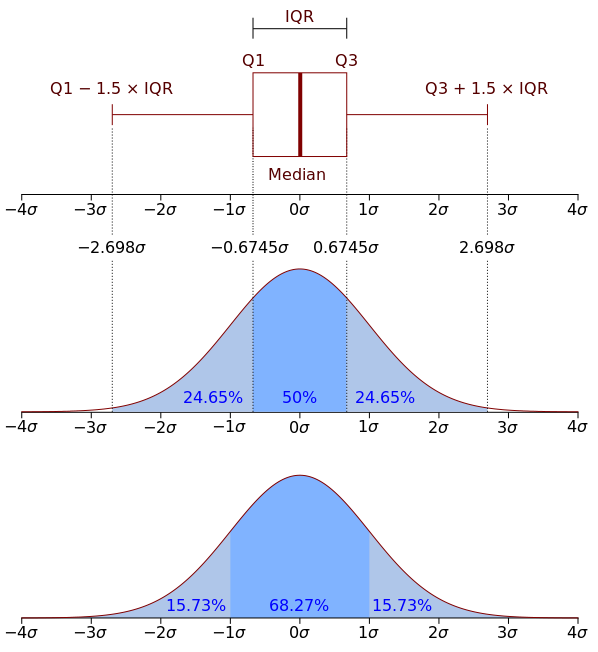
\includegraphics[width=0.7\textwidth]{figures/chapter4/surrogates/Boxplot_vs_PDF.png}
\caption{A plot explaining the scope of the boxplot (@TODO add this to appendix). The top plot represent the boxplot, with median in the middle. The range of the box spans from Quartile 1 to Quartile 3. The interquartile region (IQR) is the width of the box. The whiskers span from the edges of the box to length of 1.5 IQR to either side of the axis.
  The two bottom plots explain the ranges in terms of percentages and width of the distribution. Additionaly, an outlier is a value lying outside the both whiskers range. }
\label{fig:boxplot}
% source: https://towardsdatascience.com/create-and-customize-boxplots-with-pythons-matplotlib-to-get-lots-of-insights-from-your-data-d561c9883643
% source; https://commons.wikimedia.org/wiki/File:Boxplot_vs_PDF.svg
\end{figure}
